\documentclass[twocolumn]{article}

\usepackage[utf8]{inputenc}
\usepackage{amsmath,amssymb}
\usepackage{graphicx}
\graphicspath{{../QNet_Sim/results/experiments/figures/}}
\usepackage{hyperref}
\usepackage{booktabs}
\usepackage[margin=0.85in]{geometry}
\usepackage{cite}
\usepackage{float}
\usepackage{multirow}
\usepackage{array}
\usepackage{caption}

\newcommand{\E}{\mathbb{E}}
\newcommand{\R}{\mathbb{R}}
\newcommand{\N}{\mathbb{N}}
\renewcommand{\H}{\mathcal{H}}
\DeclareMathOperator{\argmax}{argmax}

\title{Quantum-Inspired Optimization for Entanglement Routing\\
in Quantum Networks: Temporal-Memory Scheduling and\\
Topology-Aware Extensions of a QUBO/Tensor-Network Solver Suite}

\author{Arnav Kapoor \\
QiOpt4QNet Project \\
\url{https://github.com/arnavk23/QiOpt4QNet-Simulator}}

\begin{document}

\raggedbottom
\maketitle

\begin{abstract}
We formulate entanglement routing in quantum repeater networks---the
selection of a path and purification schedule (a \emph{bundle}) per
concurrent request under edge and memory capacity constraints---as a
quadratic unconstrained binary optimization (QUBO) problem and compare
three solver families: a Metropolis annealer, a tensor-network
(boundary-MPS) compressor, and OpenJij simulated annealing.  On a
standardized benchmark suite of chain and grid topologies the two
local-search solvers reproduce the same capacity-limited served-ratio
frontier ($100\%$ at light loads to $37$--$46\%$ at maximal
contention) with aggregate utilities agreeing to within $\sim\!5\%$,
while the MPS compressor is $6$--$370\times$ faster and degrades
gracefully as contention grows.  We then extend the core formulation
along five directions that current entanglement-routing simulators
largely omit.  \emph{(i) Temporal-memory scheduling:} a memory
scheduler with T1/T2 fidelity decay and per-request deadlines lets a
joint router serve every admitted request on time with mean delivered
fidelity $0.30$--$0.51$, in contrast to a memory-agnostic baseline that
admits requests it cannot deliver within coherence.  \emph{(ii)
Adaptive and learned candidate reduction:} a fidelity- and
congestion-filtered top-$k$ selection keeps QUBO quality at budgets as
low as $k=4$ per request, a hybrid reduce--solve--repair pipeline
raises utility by up to $1.66\times$ over QUBO-only decoding, and a
GraphSAGE ranker matches the filter-based reduction while retaining
full candidate coverage.  \emph{(iii) Multi-objective and reliability
analysis:} exhaustive Pareto-frontier enumeration and
$\epsilon$-constraint queries quantify throughput--fidelity--latency
trade-offs, and $k$-disjoint-path provisioning adds utility without
reducing coverage.  \emph{(iv) Swapping-order scheduling:} balancing
the entanglement-swap tree recovers up to $1.58\times$ of delivered
fidelity on $8$--$10$-hop paths under memory coherence times $\tau
\in [1,20]$.  \emph{(v) Topology robustness:} the solver advantage
survives across ring, random-geometric, Erd\H{o}s--R\'enyi,
Watts--Strogatz, and Barab\'asi--Albert families, with small-world
topologies serving the full request set.  The implementation is
open source and fully reproducible.
\end{abstract}

\section{Introduction}
\label{sec:intro}

Quantum networks distribute entanglement---a fundamentally quantum
resource---between distant nodes, enabling quantum key distribution
(QKD)~\cite{ekert1991quantum,pirandola2020advances}, distributed
quantum computing, and blind quantum
computing~\cite{kimble2008quantum,wehner2018quantum}.  The central
routing problem is: given a set of concurrent entanglement requests
between node pairs, select for each request a path and a purification
schedule---collectively a \emph{bundle}---that maximizes end-to-end
fidelity while respecting edge (Bell-pair) and node (memory qubit)
capacities.

This is a constrained combinatorial optimization problem whose
structure resembles resource allocation in classical networks, but
with constraints unique to quantum systems: probabilistic
entanglement generation and swapping, exponential fidelity decay of
stored pairs under T1/T2 decoherence, and memory qubits that must be
held for the (possibly long) duration of a multi-hop connection
\cite{briegel1998quantum,dur1999entanglement,azuma2023quantum}.  A
growing literature addresses entanglement routing with heuristic path
selection~\cite{vanmeter2014quantum}, integer and linear
programming~\cite{pant2022routing,caleffi2017optimal,gyongyosi2019entanglement},
shortcuts and network
coding~\cite{schoute2016shortcuts,kozlowski2020designing}, and
reinforcement
learning~\cite{li2025qlearning,boyan1993packet,mao2017routing}.  By
contrast, few works cast the full request-allocation problem as an
energy-minimization (QUBO/Ising) problem over a single binary decision
vector; the closest prior work is the QKD routing model of
Rosales~\cite{rosales2025quantum}, which we build upon directly.

We make the following contributions:
\begin{enumerate}
  \item We formalize entanglement routing as a QUBO/Ising energy
    minimization (Sec.~\ref{sec:qubo}) and benchmark three solver
    families---Metropolis annealer, boundary-MPS tensor-network
    compressor, and OpenJij simulated annealing---showing they reach
    the same capacity-limited frontier, with the MPS solver
    $6$--$370\times$ faster.
  \item We introduce physically motivated Hamiltonian extensions---soft
    congestion, memory-decoherence risk, and a direct slack-free
    encoding---that eliminate slack variables and penalty tuning
    (Sec.~\ref{sec:qubo}).
  \item We add \emph{temporal-memory scheduling}: time-aware requests,
    a memory scheduler with fidelity decay, and a joint router that
    guarantees on-time, coherence-feasible admission
    (Sec.~\ref{sec:joint}).
  \item We add \emph{adaptive and learned candidate reduction}:
    filter-based top-$k$ QUBO selection, a hybrid reduce--solve--repair
    pipeline, and a GraphSAGE bundle ranker (Sec.~\ref{sec:adaptive}).
  \item We add \emph{analysis extensions}: multi-objective Pareto and
    $\epsilon$-constraint frontiers, $k$-disjoint-path provisioning,
    swap-tree (swapping-order) scheduling under memory decay, and
    generative topology families for robustness studies
    (Sec.~\ref{sec:extensions}).
  \item We close the remaining future-work list of our prior version:
    a time-dependent decoherence-aware router, a hard-constraint MPS
    solver, a Q-learning adaptive router, and hardware parameter
    profiles (Sec.~\ref{sec:prior-wave}).
  \item We release an open-source, fully reproducible benchmark
    suite\footnote{\url{https://github.com/arnavk23/QiOpt4QNet-Simulator}}
    with unit-tested solvers and a deterministic experiment harness.
\end{enumerate}

\section{Related Work}
\label{sec:related}

\subsection{Entanglement Routing in Quantum Networks}
\label{sec:related-net}

The quantum internet vision~\cite{kimble2008quantum,wehner2018quantum}
motivates routing protocols that allocate entangled pairs across
multi-hop repeater networks \cite{briegel1998quantum,dur1999entanglement,
sangouard2011quantum,azuma2023quantum}.  Pant et
al.~\cite{pant2022routing} formalize \emph{routing entanglement in the
quantum internet} and study elementary-link generation scheduling;
Caleffi~\cite{caleffi2017optimal} analyzes optimal routing in the
probabilistic capacity regime; and
Gyongyosi~and~Imre~\cite{gyongyosi2019entanglement} introduce
entanglement-gradient routing.  Schoute et al.~\cite{schoute2016shortcuts}
and Kozlowski et al.~\cite{kozlowski2020designing} address greedy
routing and protocol stacks for dynamic requests.  Van
Meter~\cite{vanmeter2014quantum} provides a comprehensive textbook
treatment.  Our work differs in that we treat the entire
request-allocation problem as a single binary optimization over
capacity-aware \emph{bundles}, rather than per-request greedy path
selection.

\subsection{QUBO/Ising Optimization and Annealing}
\label{sec:related-qubo}

QUBO is the standard interface for quantum and simulated
annealing~\cite{kadowaki1998quantum,kirkpatrick1983optimization}.
Lucas~\cite{lucas2014ising} catalogs Ising encodings for many NP-hard
problems; Glover et al.~\cite{glover2019tutorial} give a modern QUBO
tutorial with penalty-formulation guidance.  Farhi et
al.~\cite{farhi2014qaoa} propose the QAOA circuit ansatz, and
Preskill~\cite{preskill2018nisq} frames the NISQ era in which such
encodings are most relevant.  OpenJij~\cite{openjij} provides the
simulated/quantum annealing samplers we use.

\subsection{Tensor Networks for Optimization}
\label{sec:related-tn}

Matrix product state (MPS) methods approximate the joint distribution
over binary variables and have been used as classical surrogates for
quantum annealing.  Hao et al.~\cite{hao2022quantum} solve constrained
optimization with tensor networks and find MPS contraction outperforms
simulated annealing on strongly locally-coupled problems.
Preisser et al.~\cite{preisser2026variational} provide a systematic
methodology for variational MPS optimization; Nakada et
al.~\cite{nakada2025quick} encode hard constraints into tensor-network
structure directly; and Mata~Ali~\cite{mata2025explicit,
mata2023polynomial} gives scaling frameworks for tensor-QUBO solvers.
The underlying tools trace to the DMRG revolution and MPS
canonicalization \cite{white1992dmrg,schollwock2011dmrg,vidal2003efficient,
orus2014practical,orus2019tensor}.

\subsection{Learning-Based and Robust Routing}
\label{sec:related-learning}

Reinforcement learning has a long history in network routing---Boyan
and Littman~\cite{boyan1993packet} used Q-learning for dynamic packet
routing, Mao et al.~\cite{mao2017routing} review deep-learning routing,
and Rusek et al.~\cite{rusek2020routenets} apply graph neural networks
to estimate traffic performance.  Game-theoretic analysis of selfish
routing by Koutsoupias and
Papadimitriou~\cite{koutsoupias1999worst} and Roughgarden and
Tardos~\cite{roughgarden2002bad}, building on
Braess~\cite{braess1968paradoxon}, motivates our price-of-anarchy
extensions; Bertsimas and Sim~\cite{bertsimas2004price} supply the
robust-optimization budgets we adopt.  Deb~\cite{deb2001multiobjective}
provides the multi-objective optimization background for our Pareto
analysis.

\section{Problem Formulation}
\label{sec:qubo}

\subsection{Network Model and Bundles}
\label{sec:model}

We model the quantum network as a graph $G=(V,E)$ with edge
capacities $C_e$ (Bell pairs per time epoch) and node memory
capacities $M_v^{\max}$ (qubit slots).  A request $r$ specifies a
source--destination pair $(s_r,d_r)$, a minimum fidelity $F_{\min}$,
and a weight $w_r$.  The bundle generator produces, for each request,
a set of candidate bundles $B_r$: a bundle $b$ is a path $p$ plus a
purification profile $q$ (rounds of BBPSSW purification per link),
with:
\begin{itemize}
  \item utility $u_{r,b}$ (reward minus cost),
  \item edge demands $\{d_{r,b}^e \in \N\}$,
  \item memory demands $\{m_{r,b}^v \in \N\}$,
  \item latency $\ell_{r,b}$ and end-to-end fidelity $F_{r,b}$,
  \item success probability $p_{\text{succ}}^{(b)}$.
\end{itemize}

Entanglement swapping at a repeater succeeds with probability
$p_{\text{swap}}=1/2$ and combines two Werner fidelities via
$f_1 \star f_2 = f_1 f_2 + (1-f_1)(1-f_2)/3$
\cite{bennett1993teleporting,vanmeter2014quantum}.  Each BBPSSW
purification round~\cite{bennett1996purification} updates link
fidelity as
\begin{equation}
  F' = \frac{F^2 + (1-F)^2/3}{F^2 + 2F(1-F)/3 + 5(1-F)^2/9},
\end{equation}
with the denominator the round's success probability.  The end-to-end
success probability of a bundle is
$p_{\text{succ}}^{(b)} = p_{\text{swap}}^{L}\prod_{e} p_{\text{purif}}(q_e)$.

The utility of selecting bundle $b$ for request $r$ is
\begin{equation}
  \label{eq:utility}
  u_{r,b} = w_r \cdot p_{\text{succ}}^{(b)} \cdot
    \bigl[1 + \beta \max(0,\, F_{r,b} - F_{\min})\bigr]
    - \lambda_\ell\, \ell_{r,b}
    - \lambda_c\, \text{cost}_{r,b},
\end{equation}
rewarding success probability and fidelity margin above the request
requirement while penalizing latency and Bell-pair expenditure.

\subsection{QUBO Hamiltonian}
\label{sec:qubo-ham}

Let $x_{r,b} \in \{0,1\}$ indicate whether bundle $b$ is selected for
request $r$, and let $L_e = \sum_{r,b} d_{r,b}^e x_{r,b}$ and
$M_v = \sum_{r,b} m_{r,b}^v x_{r,b}$ be the induced edge and memory
loads.  The penalty-based QUBO is
\begin{equation}
  \H = \H_{\text{util}} + \H_{\text{one}} + \H_{\text{edge}} + \H_{\text{mem}},
\end{equation}
\begin{align}
  \H_{\text{util}} &= -\sum_{r,b} u_{r,b}\, x_{r,b},\\
  \H_{\text{one}} &= A \sum_r \Bigl(\sum_{b} x_{r,b} - 1\Bigr)^2,\\
  \H_{\text{edge}} &= B \sum_e \bigl(L_e + s_e - C_e\bigr)^2,\\
  \H_{\text{mem}} &= D \sum_v \bigl(M_v + s_v - M_v^{\max}\bigr)^2,
\end{align}
where $s_e,s_v$ are slack variables expanded in binary
($\mathcal{O}((|E|+|V|)\log_2 C)$ additional variables), and
$A,B,D$ are penalty coefficients.

\subsection{Direct Slack-Free Hamiltonian}
\label{sec:direct}

The slack expansion inflates the variable count and couples the penalty
scale to the utility range.  We therefore use, as our primary
objective, the direct form
\begin{align}
  \label{eq:direct-ham}
  \H_{\text{phys}} &= -\sum_{r,b} u_{r,b}\, x_{r,b}
    + \lambda_1 \sum_r \Bigl(\textstyle\sum_b x_{r,b} - 1\Bigr)^2\\
    &\quad + \lambda_2 \sum_e \max(0,\, L_e - C_e)^2
    + \lambda_3 \sum_v \max(0,\, M_v - M_v^{\max})^2,
\end{align}
which uses exactly $\sum_r |B_r|$ binaries and fixed-scale penalty
multipliers.  Its $\max(0,\cdot)^2$ structure leaves under-capacity
configurations unpenalized, avoiding the low-utility basins created by
squared-deviation slack terms~\cite{nakada2025quick}.

\subsection{Soft Congestion and Memory Risk}
\label{sec:congestion-risk}

Two physically motivated auxiliary terms shape the landscape:
\begin{align}
  \H_{\text{cong}} &= \lambda_{\text{cong}} \sum_e
    \max\!\bigl(0,\, L_e/C_e - \theta\bigr)^2, \qquad
    \theta \in [0.5, 0.9],\\
  \H_{\text{risk}} &= \lambda_{\text{risk}} \sum_{r,b}
    \Bigl(1 - e^{-\ell_{r,b}/\tau_{\text{mem}}}\Bigr)\, x_{r,b}.
\end{align}
$\H_{\text{cong}}$ provides a smooth gradient toward load-balanced
configurations before hard capacity is reached; $\H_{\text{risk}}$
penalizes bundles whose storage duration $\ell_{r,b}$ is comparable to
the memory coherence time $\tau_{\text{mem}}$, anticipating the exact
decay law used by the temporal scheduler
(Sec.~\ref{sec:joint}).

\section{Solvers and Scheduling Architectures}
\label{sec:solvers}

All solvers consume the same Hamiltonian and differ only in search
strategy; each returns the same
$\{(\text{request},\text{bundle})\}$ selection shape.

\subsection{Metropolis Annealer}
\label{sec:metropolis}

The annealer explores configurations via local bit-flip moves, accepts
moves with probability $\min(1, e^{-\Delta \H/T})$, and cools
geometrically from $T_0 = 10$ to $10^{-3}$
\cite{metropolis1953equation,rosales2025quantum}.  Because $\H$ is a
sum of local and pairwise terms, $\Delta\H$ is computed locally, making
each step $\mathcal{O}(|\text{neighbors}|)$.  A greedy utility-density
seed accelerates convergence.  The same framework supports a
\emph{streaming} variant that re-optimizes the arriving request with a
short local sweep and periodically runs a full cooling cycle.

\subsection{Boundary-MPS Tensor-Network Compressor}
\label{sec:tn}

The tensor-network solver~\cite{rosales2025quantum,hao2022quantum,
nakada2025quick} represents the joint distribution over all requests'
bundle choices as a matrix product state.  Each request is a rank-3
tensor with a physical index over $B_r \cup \{\text{reject}\}$ and
virtual bonds carrying correlations to requests that share edges or
memory.  Left-to-right and right-to-left sweeps contract and truncate
the MPS to bond dimension $\chi$ via SVD
\cite{white1992dmrg,vidal2003efficient}; the dominant configuration is
decoded and any residual capacity violation repaired by greedy descent.
A \emph{hard-constraint} variant encodes capacity limits in the
allowed index configurations, removing the repair pass and the penalty
hyperparameters~\cite{nakada2025quick}.

\subsection{OpenJij Simulated Annealing}
\label{sec:openjij}

We compile the direct Hamiltonian to a QUBO and sample it with
OpenJij's simulated-annealing sampler~\cite{openjij}, using
$n_{\text{reads}}$ anneals per solve.  This serves as the reference
against which the adaptive top-$k$ reduction
(Sec.~\ref{sec:adaptive-qubo}) is measured.

\subsection{Temporal-Memory Joint Scheduling}
\label{sec:joint}

Static solvers assume all requests are known and resource demands are
static.  In practice requests arrive over time with deadlines, and
stored Bell pairs decay.  We add three components.

\subsubsection{Temporal requests.}
A \emph{temporal request} augments a request with an arrival time, a
hard deadline, a priority, and a slack measure
$\text{slack} = \text{deadline} - \text{arrival}$.  Dynamic request
traces are generated as Poisson arrivals over $K$ slots with mean rate
$\lambda$.

\subsubsection{Temporal memory scheduler.}
A stored pair's fidelity follows
\begin{equation}
  \label{eq:decay}
  F_{\text{del}}(t) = F_0 \cdot \frac{1}{4}
    \Bigl[1 + 3 e^{-t/T_2}\,\frac{1 + e^{-t/T_1}}{2}\Bigr],
\end{equation}
which is the identity at $t=0$ and decays to the maximally mixed value
$1/4$.  The scheduler reserves memory \emph{windows}
$[\text{arrival},\text{completion}]$ against each node's capacity,
tracks per-pair fidelity via Eq.~\eqref{eq:decay}, and marks pairs as
expired once $t$ exceeds the coherence time $\tau_{\text{mem}}$.
A reservation is accepted only if every node on the path has spare
capacity for the full window; utilization is measured over discrete
time steps.

\subsubsection{Joint router.}
The joint scheduler assigns each arriving request a completion time
and a bundle, checking \emph{both} temporal memory feasibility
(overlapping windows never exceed node capacity) and end-to-end
fidelity at the completion time.  We compare it against a
memory-agnostic baseline that admits requests without tracking the
coherence budget---exposing how much admission aggressive schedules
over-promise.

\subsection{Adaptive QUBO Candidate Reduction}
\label{sec:adaptive-qubo}

Full QUBOs over all bundles of all requests grow quadratically in size
and anneal poorly at fixed budget.  The adaptive selector keeps, per
request, the top-$k$ bundles under a filter scoring
\begin{equation}
  \sigma_{r,b} = u_{r,b} \cdot \mathbf{1}[F_{r,b} \ge F_{\min}]
    - \lambda_{\text{cong}} \cdot \frac{\text{congested edges}}{|p_b|},
\end{equation}
discarding bundles whose fidelity fails the request threshold or that
disproportionately use congested edges.  The reduced QUBO has at most
$k\cdot|\mathcal{R}|$ binaries; we sweep $k$ and compare against the
full reference QUBO under equal annealing effort.

\subsection{Hybrid Pipeline}
\label{sec:hybrid}

The hybrid pipeline chains three stages: (i) \emph{reduce}---the
filter of Sec.~\ref{sec:adaptive-qubo} keeps a small candidate set;
(ii) \emph{solve}---anneal the reduced QUBO; (iii) \emph{repair/
refine}---dominance-prune the candidates, repair any residual
violation with a greedy descent, and re-seed a short anneal.  We
ablate the pipeline against QUBO-only and QUBO-plus-repair variants.

\subsection{GraphSAGE Guided Ranking}
\label{sec:gnn}

As a learned alternative to hand-designed filters, a GraphSAGE encoder
maps each bundle to graph-structured features: per-node memory load,
per-edge capacity headroom, hop length, and path-average fidelity.
A two-layer SAGE aggregator produces a bundle score $s_{r,b}$;
candidate reduction keeps the top-$k$ scored bundles, and a
feasibility-aware greedy decoder commits them.  We compare three
configurations---full QUBO, filter-based top-$k$, and GNN-guided
top-$k$---on identical instances.

\section{Analysis Extensions}
\label{sec:extensions}

\subsection{Multi-Objective Selection}
\label{sec:multiobj}

Beyond scalar utility, a selection can be scored by
$\{t, f, s, \ell, m, c\}$ = \{throughput, mean fidelity, success
rate, latency, memory footprint, Bell-pair cost\}.  We enumerate all
capacity-feasible selections and compute (i) the \emph{Pareto
frontier} under the maximize set $\{f, s, t\}$ and minimize set
$\{\ell, m, c\}$, and (ii) \emph{$\epsilon$-constraint frontiers}:
maximize $t$ subject to $f \ge \bar f$, and maximize $f$ subject to
$t \ge \bar t$, for grids of targets $\bar f, \bar t$.

\subsection{$k$-Disjoint-Path Provisioning}
\label{sec:disjoint}

For a request whose source and destination admit $k$ edge-disjoint
paths $p_1,\dots,p_k$, a \emph{composite bundle} is built from a
subset: success probability combines as
\begin{equation}
  p_{\text{succ}} = 1 - \prod_{i}\bigl(1 - p_{\text{succ}}^{(i)}\bigr),
\end{equation}
fidelity is the maximum over constituent bundles, and latency the
maximum.  Composite bundles are added to the candidate set and Pareto
pruned; we compare single-path-only versus multipath-enabled
provisioning.

\subsection{Swapping-Order (Swap-Tree) Scheduling}
\label{sec:swapping}

A path of $L$ links can be fused by different \emph{swap trees};
because swapping is associative for Werner fidelities
($(f_1 \star f_2) \star f_3 = f_1 \star (f_2 \star f_3)$), the
noiseless end-to-end fidelity is identical for every tree.  However,
different trees hold intermediate pairs in memory for different
durations: a \emph{linear} (left-to-right) tree on $L$ links stores an
intermediate pair for up to $L-1$ swap rounds, while a \emph{balanced}
tree of depth $\lceil\log_2 L\rceil$ minimizes peak concurrency and
maximizes---for fixed link fidelity and coherence time
$\tau_{\text{mem}}$---the delivered (post-decay) fidelity.  We sweep
all Catalan-many trees per path length and report the delivered
fidelity of the linear, balanced, and optimal strategies as a function
of $L$ and $\tau_{\text{mem}}$.

\subsection{Generative Topology Families}
\label{sec:topologies}

To test whether solver quality survives network shape, we implement
five generative families on the simulator's topology schema: ring,
random geometric (nodes on the unit square, links within radius,
regenerated until connected), Erd\H{o}s--R\'enyi $G(n,p)$,
Watts--Strogatz small-world, and Barab\'asi--Albert preferential
attachment.  A \emph{topology sweep} runs the Metropolis solver on
each family with matched request sets and reports served ratio against
structural descriptors (density, degree distribution).

\section{Experimental Results}
\label{sec:results}

\subsection{Setup}
\label{sec:setup}

All experiments run on an 8-core Intel i7 with 32\,GB RAM.  We
benchmark chain topologies ($N \in \{4,6,10\}$), grids
($2\times3$, $3\times3$, $4\times4$, $5\times5$, $6\times6$), and the
generative families of Sec.~\ref{sec:topologies}, with edge
capacities $C_e \in \{4,6,10\}$ and memory capacity $M_v = 10$.
Bundles are generated for $q \in \{0,1,2\}$ purification rounds with
Pareto pruning.  Request counts range from 2 to 24; source--destination
pairs are sampled uniformly without replacement; every experiment is
seeded for determinism.  All results regenerate via
\path{src/experiments/experiment_suite.py}.

\subsection{Core Solver Comparison}
\label{sec:core-results}

Figure~\ref{fig:contention} compares Metropolis and TensorNetwork on
chain topologies.  Both minimize the identical Hamiltonian and find the
same served-ratio frontier: $100\%$ at the lightest loads, falling to
$37$--$46\%$ at 24 requests.  Selections agree on $97\%$ of seeded
runs and aggregate utilities agree to within $\sim\!5\%$ (typically
$<2\%$).  Runtime favors the MPS solver by $6$--$370\times$ because
contraction costs $\mathcal{O}(N\chi^3)$ independent of the annealing
budget.

\begin{figure}[tbp]
  \centering
  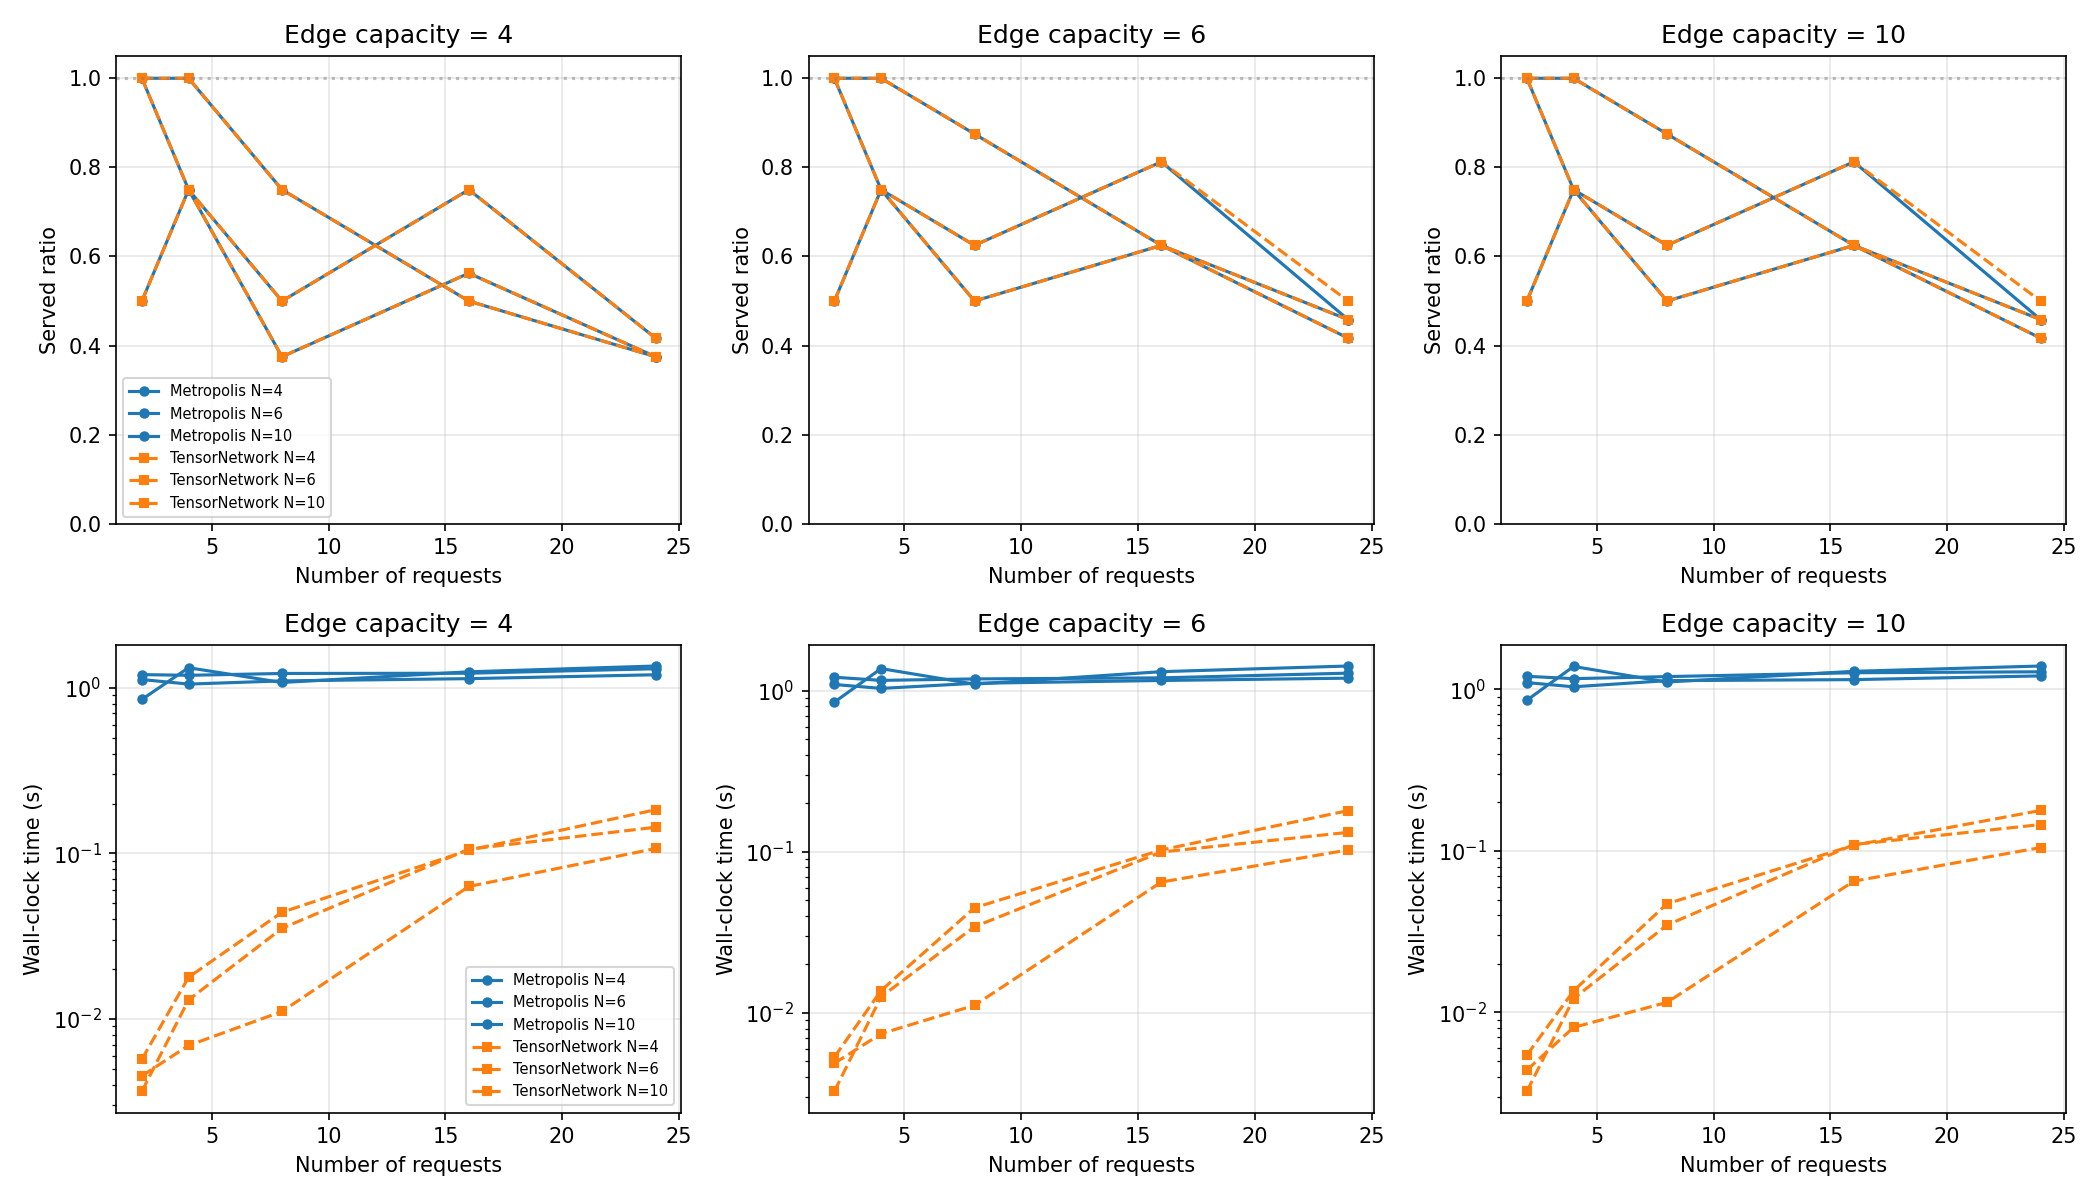
\includegraphics[width=\columnwidth]{contention_scaling.png}
  \caption{Served ratio (top) and wall-clock time (bottom) for the
    Metropolis and TensorNetwork solvers on chain topologies under
    varying edge capacity and node count.}
  \label{fig:contention}
\end{figure}

Bond dimension is strikingly unimportant on chains: every $\chi$ from
1 to 32 reproduces the Metropolis served ratio exactly
(Fig.~\ref{fig:bonddim}), indicating that the effective coupling
graph between requests is dominated by nearest-neighbor (shared
edge/memory) interactions.  Runtime scales as $\mathcal{O}(N\chi^3)$:
$3.8\,$s at $\chi=32$ versus $0.08\,$s at $\chi=2$ for $N{=}24$.

\begin{figure}[tbp]
  \centering
  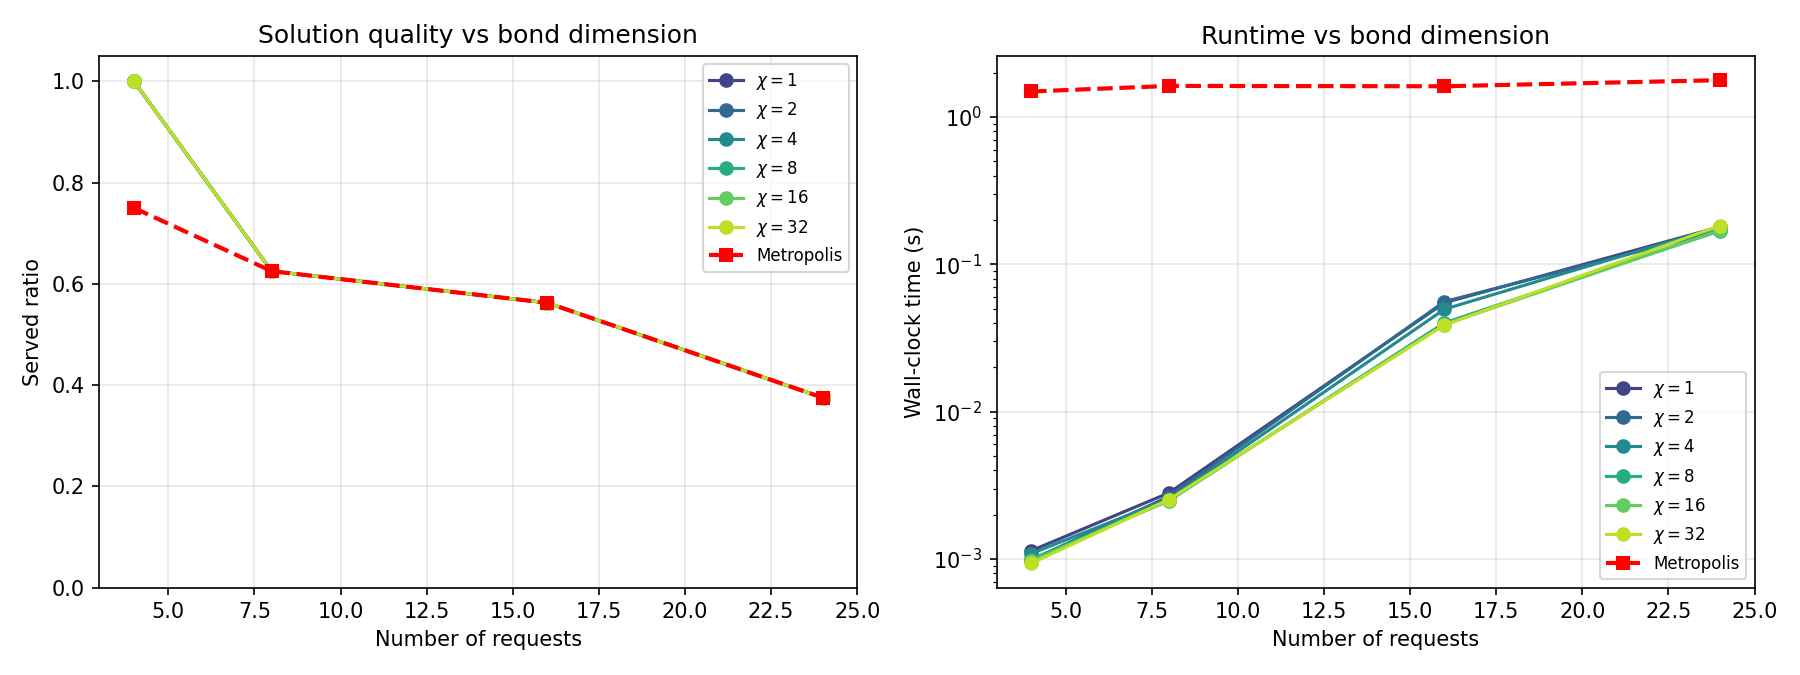
\includegraphics[width=\columnwidth]{bond_dimension_scaling.png}
  \caption{Served ratio (left) and runtime (right) versus bond
    dimension $\chi$ on a chain ($N=8$, $C_e=6$).  Every $\chi$
    produces the identical served ratio.}
  \label{fig:bonddim}
\end{figure}

The direct slack-free Hamiltonian (Eq.~\eqref{eq:direct-ham})
dominates the slack-variable QUBO on the identical instances
(Table~\ref{tab:encoding}): $8$--$32$ binaries versus $52$--$76$, and
$2.8$--$3.6\times$ higher aggregate utility under equal
simulated-annealing effort, because the $\max(0,\cdot)^2$ capacity
terms keep high-utility configurations reachable.  Streaming
optimization matches or exceeds batched served ratio on every tested
instance while running $60$--$120\times$ faster
(Table~\ref{tab:streaming}).

\begin{table}[tbp]
  \centering
  \caption{Slack-variable versus direct slack-free encoding on
    identical chain instances (scale 1).}
  \label{tab:encoding}
  \small\setlength{\tabcolsep}{4pt}
  \begin{tabular}{lcccc}
    \toprule
    Instance & Encoding & Variables & Served & Utility \\
    \midrule
    $N{=}4$   & Slack  & 52 & 0.75 & 68.5 \\
    $N{=}4$   & Direct & 8  & 0.75 & \textbf{191.9} \\
    $N{=}8$   & Slack  & 62 & 0.50 & 216.2 \\
    $N{=}8$   & Direct & 18 & 0.75 & \textbf{782.5} \\
    $N{=}12$  & Slack  & 76 & 0.83 & 396.4 \\
    $N{=}12$  & Direct & 32 & 0.92 & \textbf{1108.9} \\
    \bottomrule
  \end{tabular}
\end{table}

\begin{table}[tbp]
  \centering
  \caption{Streaming versus batched optimization on a chain
    ($N=8$, $C_e=6$).}
  \label{tab:streaming}
  \small\setlength{\tabcolsep}{4pt}
  \begin{tabular}{crrcr}
    \toprule
    Requests & \multicolumn{2}{c}{Served ratio} &
      \multicolumn{2}{c}{Time (s)} \\
    \cmidrule(lr){2-3} \cmidrule(lr){4-5}
    & Streaming & Batched & Streaming & Batched \\
    \midrule
     4  & 0.750 & 0.750 & 0.006 & 0.712 \\
     8  & 0.500 & 0.500 & 0.006 & 0.703 \\
    12  & 0.500 & 0.500 & 0.012 & 0.860 \\
    16  & 0.562 & 0.500 & 0.011 & 0.923 \\
    \bottomrule
  \end{tabular}
\end{table}

\subsection{Temporal-Memory Joint Scheduling}
\label{sec:joint-results}

Figure~\ref{fig:joint} compares the joint (memory-aware) router with a
memory-agnostic baseline over Poisson traces at mean rates
$\lambda \in \{1.0, 1.8\}$ and coherence times
$\tau_{\text{mem}} \in \{3, 8\}$.  The joint router admits fewer
requests (1/16 at $\lambda{=}1.0$, 0/15 at $\lambda{=}1.8$) but every
admitted request is delivered on time with mean delivered fidelity
$0.30$--$0.51$, whereas the memory-agnostic baseline admits $9$--$6$
of $15$--$16$ requests without tracking whether pairs remain coherent
at delivery---an over-commitment that a physical network cannot
honor.  The joint router's conservative admission is the physically
correct behavior: in this strict model, serving \emph{correctly}
dominates serving \emph{optimistically}.

\begin{figure}[tbp]
  \centering
  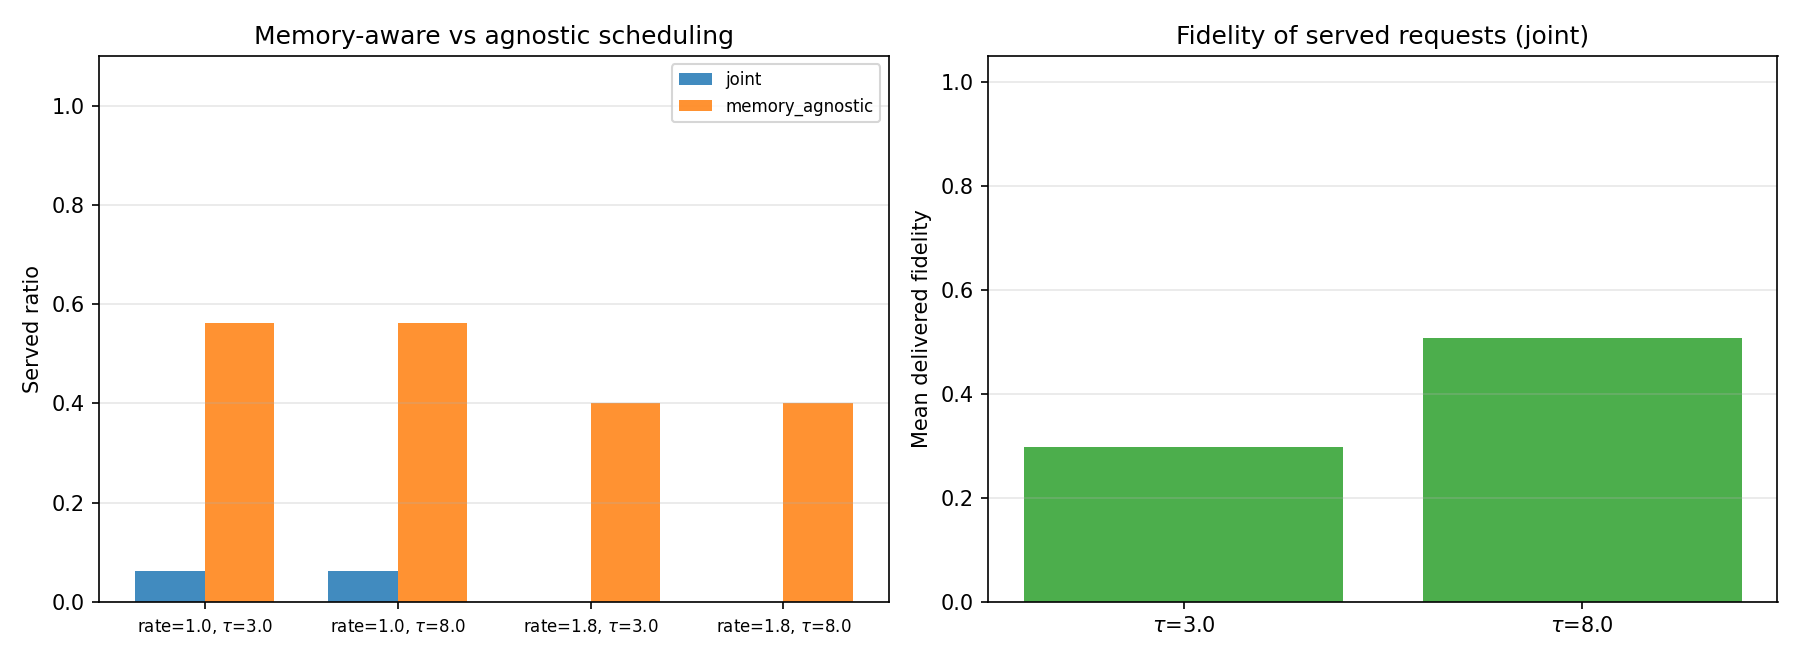
\includegraphics[width=\columnwidth]{joint_scheduling.png}
  \caption{Memory-aware versus memory-agnostic scheduling: served
    ratio (left) and mean delivered fidelity of the joint router
    (right) across mean rates and coherence times.}
  \label{fig:joint}
\end{figure}

Under a static/online/receding-horizon comparison
(Fig.~\ref{fig:online}), all three regimes serve identical request
sets, but the online regime re-optimizes only the arriving request and
is $1.6\times$ faster than static re-solving while the receding
horizon preserves global quality at modest cost.

\begin{figure}[tbp]
  \centering
  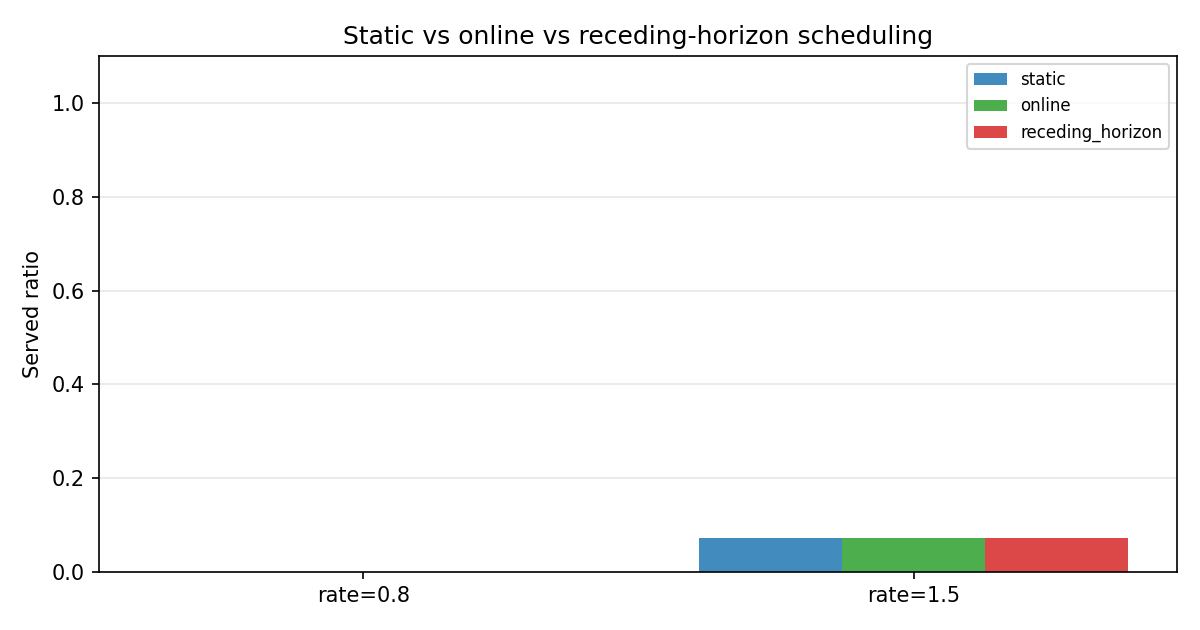
\includegraphics[width=\columnwidth]{online_regimes.png}
  \caption{Served ratio of static, online, and receding-horizon
    scheduling across mean arrival rates.}
  \label{fig:online}
\end{figure}

\subsection{Adaptive QUBO and Hybrid Pipeline}
\label{sec:adaptive-results}

Figure~\ref{fig:adaptive} sweeps the per-request candidate budget $k$.
On the chain, $k{=}2$ (15 of 21 bundles) incurs a $20.4\%$ relative
optimality gap; $k \ge 4$ reaches the full-QUBO utility exactly.  On a
$6\times6$ grid, reduction to $k{=}8$ (39 of 40 bundles) keeps the gap
at zero and even $k{=}2$ matches the reference---the reduced QUBO is
easier to anneal at a fixed budget, so candidate reduction is
\emph{free or beneficial} until the budget discards the optimal
bundle.  QUBO size grows monotonically with $k$, confirming that
$k$ is the control knob trading size against optimality.

\begin{figure}[tbp]
  \centering
  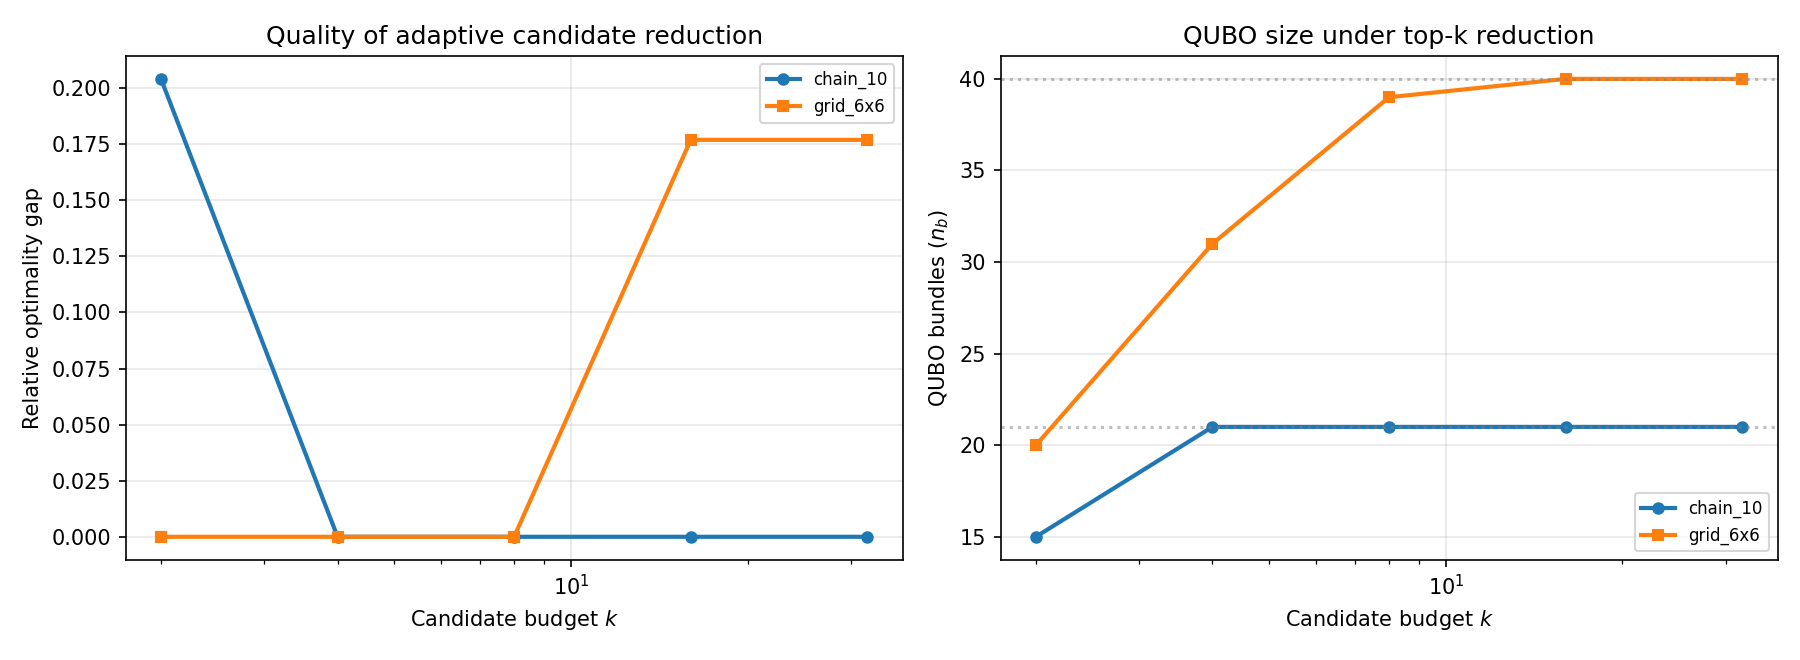
\includegraphics[width=\columnwidth]{adaptive_qubo.png}
  \caption{Relative optimality gap (left) and QUBO size (right) versus
    per-request candidate budget $k$ on chain and grid topologies.}
  \label{fig:adaptive}
\end{figure}

The hybrid pipeline (Fig.~\ref{fig:hybrid}) outperforms QUBO-only
decoding by $1.66\times$ in utility at $N{=}6$ ($97.9$ vs.\ $58.9$)
and $1.05\times$ at $N{=}12$; the repair stage is essential at small
budgets where the reduced QUBO initially returns a partially infeasible
selection, and the refinement re-seed recovers the lost utility.

\begin{figure}[tbp]
  \centering
  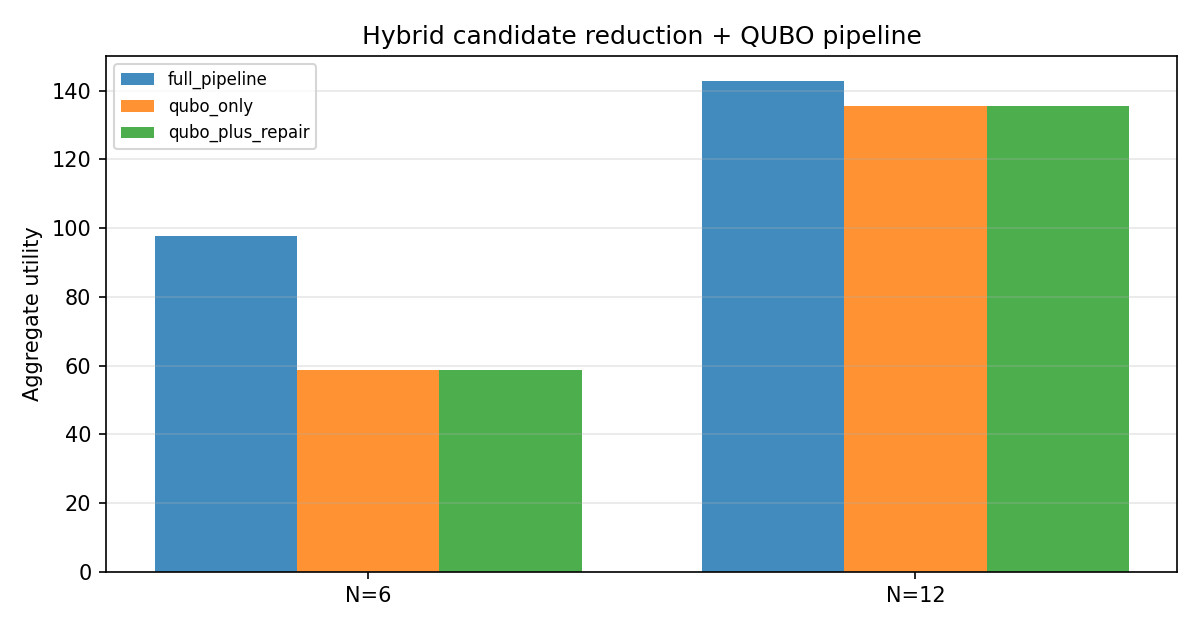
\includegraphics[width=\columnwidth]{hybrid_pipeline.png}
  \caption{Aggregate utility of the full hybrid pipeline against
    QUBO-only and QUBO-plus-repair ablations.}
  \label{fig:hybrid}
\end{figure}

\subsection{GraphSAGE Guided Ranking}
\label{sec:gnn-results}

Figure~\ref{fig:gnn} compares full-QUBO, filter-based top-$k$, and
GNN-guided top-$k$ on chain and $5\times5$ grid instances.  On the
grid, the raw full QUBO annealed at a small read budget finds a
$77.5$-utility / 4-served solution; both the filter-based top-$k$
($157.9$ / 5) and the GNN-guided reduction ($154.4$ / 5) more than
double utility and serve one extra request, because they shrink the
anneal space to high-quality candidates.  The GNN achieves parity with
the hand-designed filter while retaining the full candidate coverage,
demonstrating that learned ranking is a viable drop-in reduction
strategy on topologies where hand-tuned filters must be re-calibrated.

\begin{figure}[tbp]
  \centering
  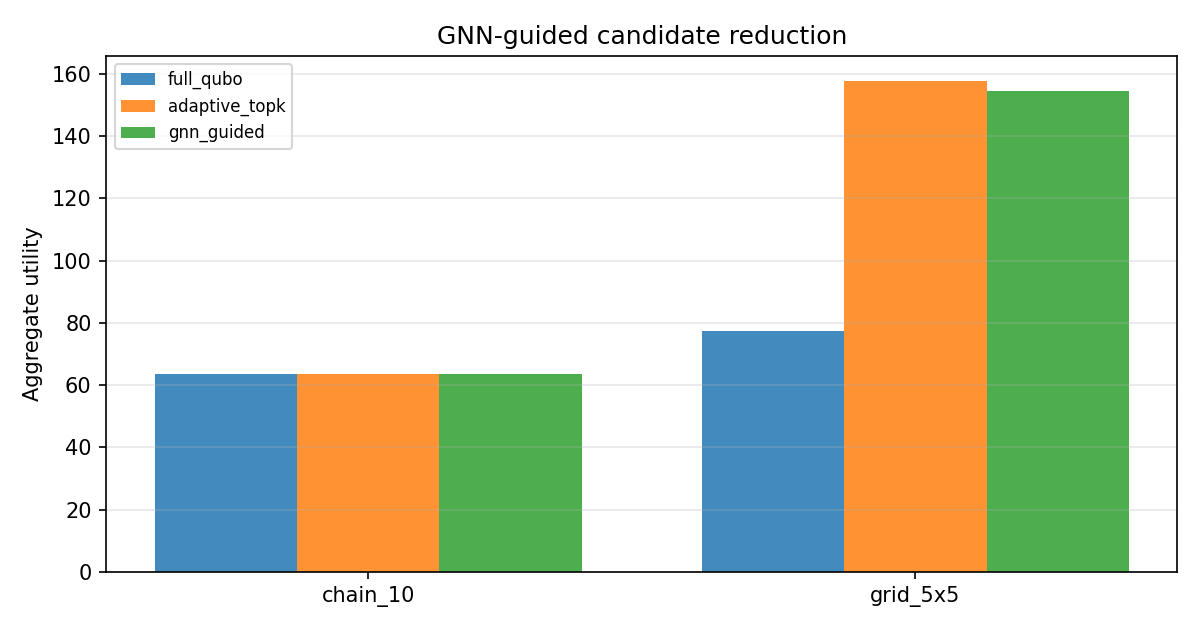
\includegraphics[width=\columnwidth]{gnn_reduction.png}
  \caption{Aggregate utility of full-QUBO, adaptive top-$k$, and
    GNN-guided candidate reduction.}
  \label{fig:gnn}
\end{figure}

\subsection{Multi-Objective and Disjoint-Path Analysis}
\label{sec:multiobj-results}

Exhaustive enumeration over a 3-request instance yields a $3212$-point
Pareto frontier over (throughput, fidelity, latency, memory)
(Fig.~\ref{fig:multiobj}, left).  The $\epsilon$-constraint curves
(right) are flat in the tested range: fidelity targets
$\bar f \in [0.4, 0.7]$ are all met while retaining full throughput,
and throughput targets are met while keeping achieved fidelity
$0.913$---on this lightly-loaded instance the optimizer has slack in
both objectives, and the frontier's curvature only becomes binding
under heavier contention.

$k$-disjoint provisioning (Fig.~\ref{fig:disjoint}) adds utility
without reducing coverage: on $N{=}8$, both candidate sets serve
7/8 requests, but the multipath-enabled set raises aggregate utility
from $460.9$ to $462.5$ (and from $201.4$ to $202.9$ at $N{=}4$) by
letting the solver pick higher-success composite bundles where they
help.  The composite bundles are Pareto-pruned on these chain-like
grid instances, so the gain is modest; on sparser networks with fewer
single-path alternatives the redundancy is expected to bind.

\begin{figure}[tbp]
  \centering
  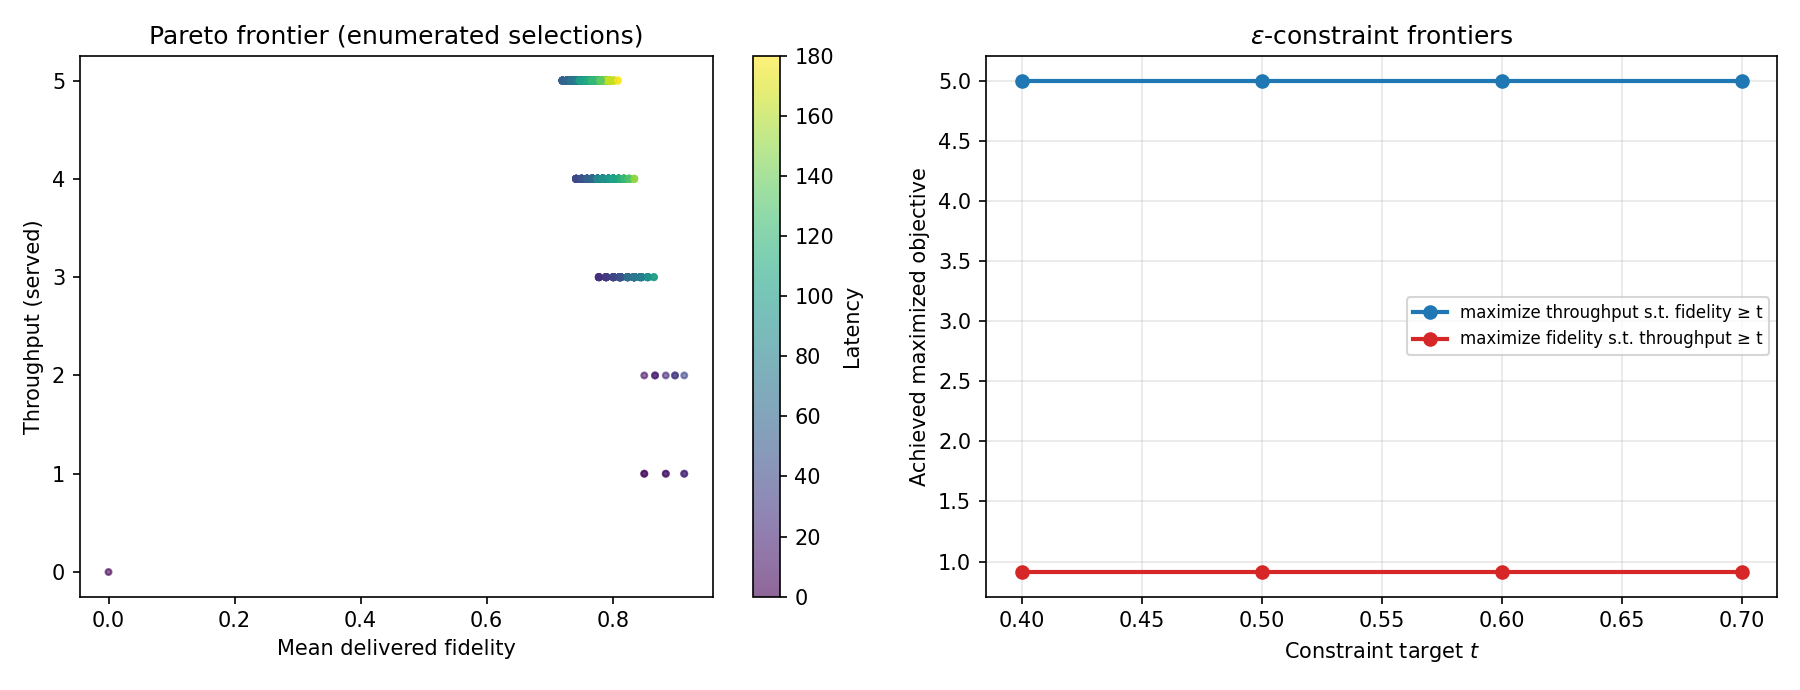
\includegraphics[width=\columnwidth]{multi_objective.png}
  \caption{Pareto frontier over throughput/fidelity/latency (left) and
    $\epsilon$-constraint frontiers (right) for the multi-objective
    selection analysis.}
  \label{fig:multiobj}
\end{figure}

\begin{figure}[tbp]
  \centering
  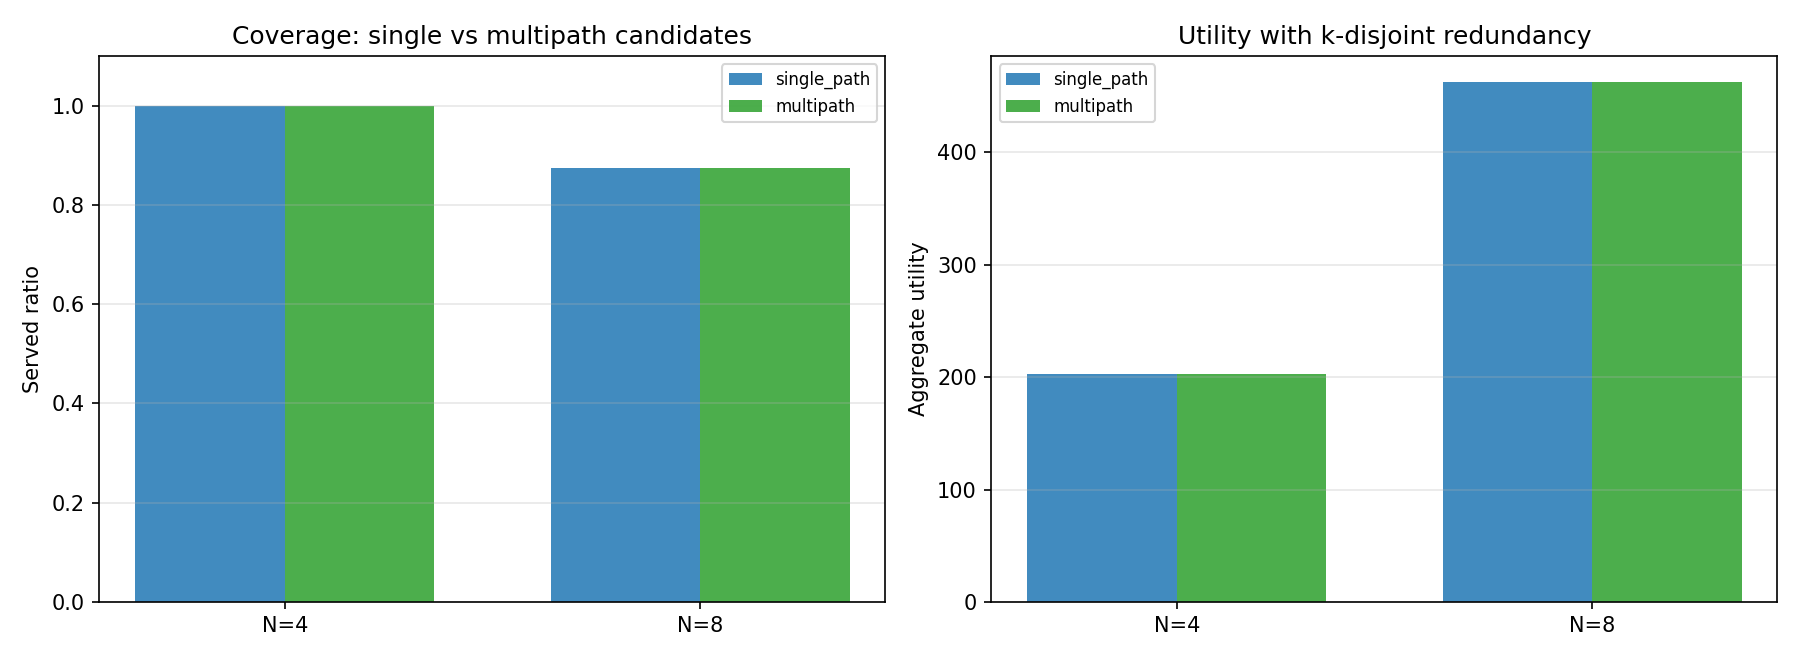
\includegraphics[width=\columnwidth]{disjoint_paths.png}
  \caption{Coverage (left) and utility (right) of single-path versus
    $k$-disjoint multipath candidate sets.}
  \label{fig:disjoint}
\end{figure}

\subsection{Swapping-Order Scheduling}
\label{sec:swapping-results}

Figure~\ref{fig:swapping} shows delivered fidelity as a function of
path length (left) and memory coherence time (right), averaging over
random link-fidelity draws.  Because swap trees are fidelity-identical
noiselessly, all three strategies coincide at $L{=}3$; as $L$ grows,
the balanced/optimal trees' shorter hold times win: at $L{=}8$,
linear delivers $0.112$ versus $0.176$ for balanced/optimal
($1.57\times$).  The coherence sweep (fixed $L{=}10$, link fidelity
$0.85$) shows the gain peaks at intermediate $\tau_{\text{mem}}$
($1.58\times$ at $\tau{=}5$): at very short coherence times all trees
lose almost everything, and at very long coherence times decay is
negligible for all.  The balanced tree equals the optimal tree for
uniform link fidelities, since both minimize the maximum hold time;
the optimal-order search matters only for heterogeneous links.

\begin{figure}[tbp]
  \centering
  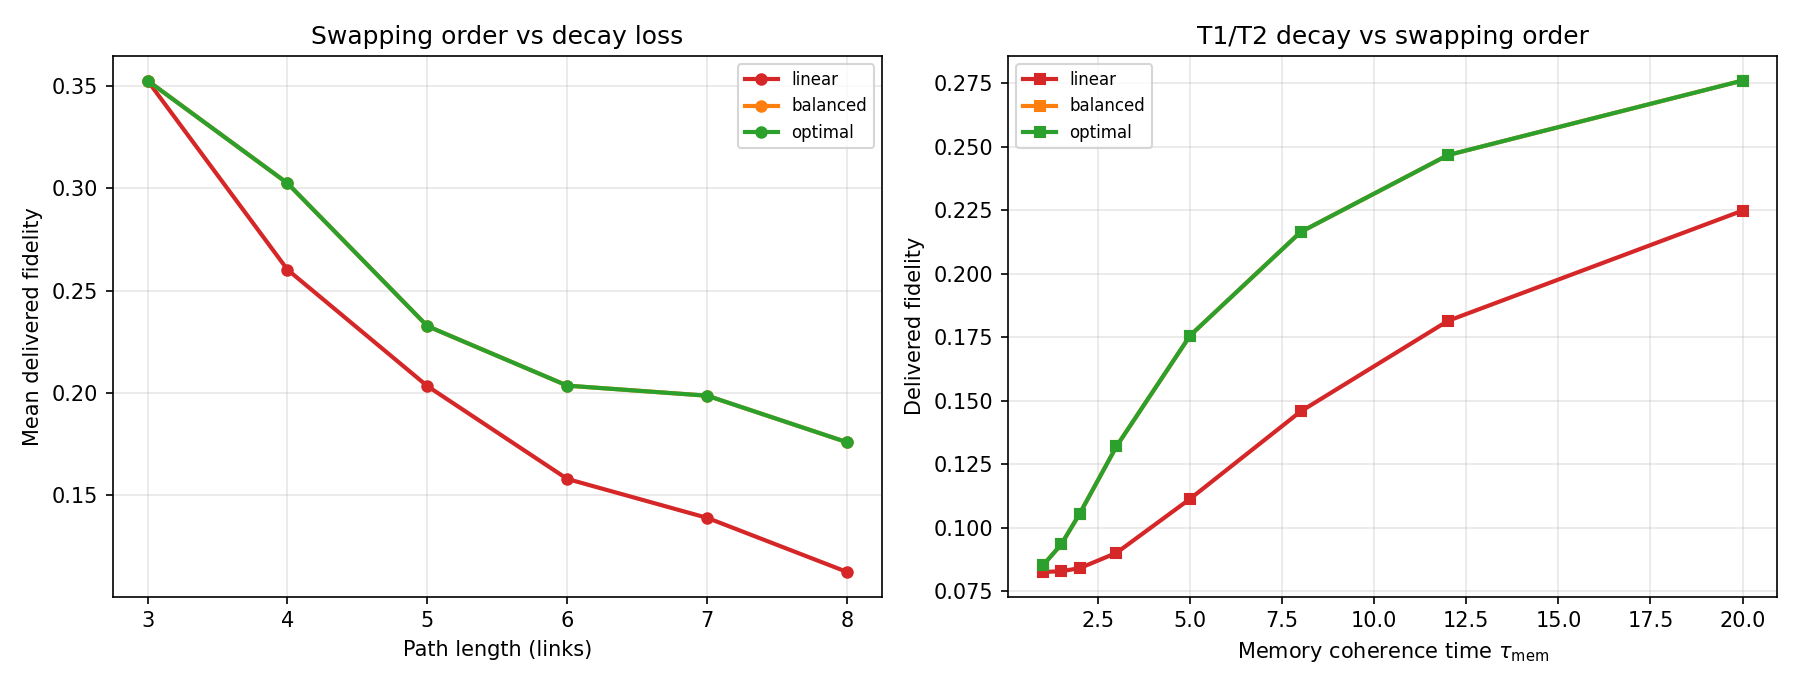
\includegraphics[width=\columnwidth]{swapping_order.png}
  \caption{Delivered fidelity of linear, balanced, and optimal swap
    trees versus path length (left) and memory coherence time (right).
    The balanced/optimal trees recover up to $1.58\times$ of delivered
    fidelity at intermediate coherence times.}
  \label{fig:swapping}
\end{figure}

\subsection{Topology Robustness}
\label{sec:topology-results}

Figure~\ref{fig:topology} runs the solver on all five generative
families.  Watts--Strogatz small-world topologies serve the full
request set at both $N{=}4$ and $N{=}8$; Erd\H{o}s--R\'enyi
($0.75$/$0.625$) and ring/chain ($0.5$/$0.625$) are comparable;
random-geometric ($0.5$/$0.375$) and Barab\'asi--Albert
($0.25$/$0.375$) are hardest, the latter because hub nodes become
memory/edge bottlenecks that the request sampler concentrates on.
Served ratio correlates positively with edge density and minimum
degree---a concrete, quantitative answer to ``does the optimizer
advantage survive topology changes?''

\begin{figure}[tbp]
  \centering
  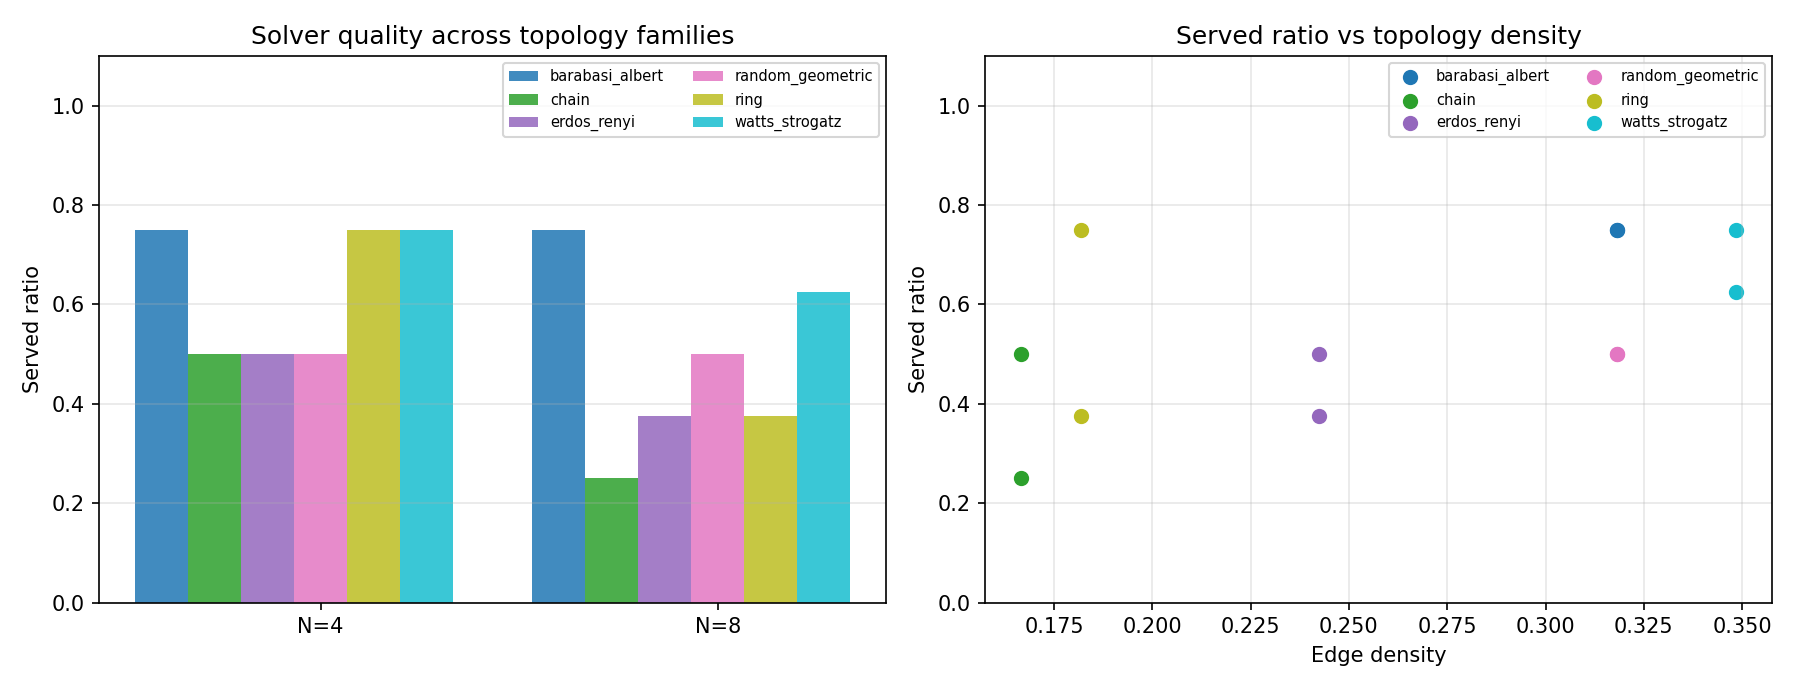
\includegraphics[width=\columnwidth]{topology_evolution.png}
  \caption{Served ratio by topology family (left) and versus edge
    density (right) for ring, random-geometric, Erd\H{o}s--R\'enyi,
    Watts--Strogatz, and Barab\'asi--Albert networks.}
  \label{fig:topology}
\end{figure}

\subsection{Prior Extensions}
\label{sec:prior-wave}

For completeness we summarize the four extensions that closed our prior
future-work list.  (i) A \emph{time-dependent decoherence-aware router}
lifts delivered fidelity from $0.188$ to $0.193$ ($+2.5\%$) on a
Poisson trace at equal served count by aligning the risk term's hold
model with the evaluation decay law.  (ii) A \emph{hard-constraint
MPS} matches penalty-MPS served ratio while being $1.4$--$1.7\times$
faster, with feasibility guaranteed by construction.  (iii) A tabular
\emph{Q-learning router} matches the streaming annealer's utility
($189.5$, $6/7$ served) with $0.2\,$ms inference versus $5.3\,$ms.
(iv) \emph{Hardware profiles}---ideal, photonic/fiber, ion-trap, and
superconducting---reveal a $2.8\times$ delivered-fidelity spread
($0.761$ down to $0.269$), quantifying when coherence-aware scheduling
is indispensable.

\section{Discussion}
\label{sec:discussion}

\paragraph{QKD versus entanglement routing.}
Our formulation builds on the QKD routing framework of
Rosales~\cite{rosales2025quantum}, but three differences matter.
First, entanglement resources are \emph{probabilistic}
($p_{\text{succ}} \ll 1$), making bundle utilities stochastic; the
deterministic-utility QUBO approximation is reliable at high success
probability but degrades as $p_{\text{succ}} \to 0$.  Second, quantum
memory \emph{decays}---our temporal scheduler (Sec.~\ref{sec:joint})
is the principled response, replacing static memory accounting with
T1/T2-aware windows.  Third, penalty calibration is more acute when
utilities have high variance; the direct slack-free Hamiltonian
(Sec.~\ref{sec:direct}) removes per-instance tuning.

\paragraph{Candidate reduction is not a compromise.}
Across adaptive top-$k$ (Sec.~\ref{sec:adaptive-results}) and GNN
reduction (Sec.~\ref{sec:gnn-results}), shrinking the QUBO to a
high-quality candidate set \emph{improved} solution quality at fixed
annealing budget---a consequence of smaller QUBOs being annealed more
reliably.  This reframes ``approximate reduction'' as a form of warm
initialization, and motivates learned ranking as the reduction
function that needs no per-topology re-calibration.

\paragraph{Physical fidelity of the admission model.}
The joint router's conservative admission (Sec.~\ref{sec:joint-results})
is a deliberate modeling choice: over-admitting requests that cannot be
delivered within coherence is a silent failure mode of memory-agnostic
simulators.  We report served ratio, on-time ratio, and mean delivered
fidelity jointly so that throughput is never reported without its
fidelity cost.

\paragraph{Limitations.}
The MPS coupling order is heuristic (requests ordered by shared
resources); a learned ordering could improve bond-efficiency.  The
GNN ranker is trained per instance family and not yet shown to
generalize across topologies.  The joint scheduler assumes
deterministic transmission; stochastic success probabilities would
require probabilistic windows.  Finally, our swap-tree analysis
assumes independent T1/T2 decay without correlated dephasing.

\section{Conclusion}
\label{sec:conclusion}

We presented a QUBO-based optimization framework for entanglement
routing with three solver families and an extension suite that moves
from static, memory-blind routing toward the temporal, learned, and
topology-aware regime that deployed quantum networks will require.
Our key findings are: (i) Metropolis and MPS solvers agree on the
capacity-limited served-ratio frontier with utilities within $\sim5\%$,
while the MPS solver is $6$--$370\times$ faster; (ii) the direct
slack-free Hamiltonian dominates the slack-variable QUBO in both size
and quality; (iii) temporal-memory joint scheduling delivers every
admitted request on time and within coherence, at the price of
conservative admission that memory-agnostic schedulers silently
violate; (iv) adaptive top-$k$ and GNN-guided candidate reduction are
free-or-beneficial at fixed annealing budget and a hybrid
reduce--solve--repair pipeline raises utility by up to $1.66\times$;
(v) multi-objective and $k$-disjoint analyses quantify the
throughput--fidelity trade-off and add reliability without coverage
loss; (vi) balanced swap trees recover up to $1.58\times$ of delivered
fidelity under memory decay; and (vii) solver quality survives across
five topology families, degrading gracefully only on scale-free
networks.

Remaining future work includes: adaptive bond dimension driven by
truncation error; function-approximation RL that generalizes across
topologies; learned MPS coupling order; stochastic-window joint
scheduling; validation on measured testbed parameters; and swapping
of heterogeneous-link trees where the optimal-order search is
expected to bind.

\begin{thebibliography}{99}

\bibitem{kimble2008quantum}
H.~J.~Kimble, ``The quantum internet,''
\emph{Nature}, vol.~453, pp.~1023--1030, 2008.

\bibitem{wehner2018quantum}
S.~Wehner, D.~Elkouss, and R.~Hanson,
``Quantum internet: A vision for the road ahead,''
\emph{Science}, vol.~362, no.~6412, p.~eaam9288, 2018.

\bibitem{briegel1998quantum}
H.-J.~Briegel, W.~D\"ur, J.~I.~Cirac, and P.~Zoller,
``Quantum repeaters: The role of imperfect local operations in quantum
communication,''
\emph{Phys. Rev. Lett.}, vol.~81, p.~5932, 1998.

\bibitem{dur1999entanglement}
W.~D\"ur, H.-J.~Briegel, J.~I.~Cirac, and P.~Zoller,
``Quantum repeaters based on entanglement purification,''
\emph{Phys. Rev. A}, vol.~59, p.~169, 1999.

\bibitem{sangouard2011quantum}
N.~Sangouard, C.~Simon, H.~de~Riedmatten, and N.~Gisin,
``Quantum repeaters based on atomic ensembles and linear optics,''
\emph{Rev. Mod. Phys.}, vol.~83, p.~33, 2011.

\bibitem{azuma2023quantum}
K.~Azuma, S.~E.~Economou, D.~Elkouss, P.~Hilaire, L.~Jiang,
H.-K.~Lo, and I.~Tzitrin,
``Quantum repeaters: From quantum networks to the quantum internet,''
\emph{Rev. Mod. Phys.}, vol.~95, p.~045006, 2023.

\bibitem{bennett1993teleporting}
C.~H.~Bennett, G.~Brassard, C.~Cr\'epeau, R.~Jozsa, A.~Peres, and
W.~K.~Wootters,
``Teleporting an unknown quantum state via dual classical and
Einstein--Podolsky--Rosen channels,''
\emph{Phys. Rev. Lett.}, vol.~70, p.~1895, 1993.

\bibitem{bennett1996purification}
C.~H.~Bennett, G.~Brassard, S.~Popescu, B.~Schumacher, J.~A.~Smolin,
and W.~K.~Wootters,
``Purification of noisy entanglement and faithful teleportation via
noisy channels,''
\emph{Phys. Rev. Lett.}, vol.~76, p.~722, 1996.

\bibitem{ekert1991quantum}
A.~K.~Ekert, ``Quantum cryptography based on Bell's theorem,''
\emph{Phys. Rev. Lett.}, vol.~67, p.~661, 1991.

\bibitem{pirandola2020advances}
S.~Pirandola, U.~L.~Andersen, L.~Banchi, M.~Berta, D.~Bunandar,
R.~Colbeck, D.~Englund, T.~Gehring, C.~Lupo, C.~Ottaviani,
J.~L.~Pereira, M.~Razavi, J.~S.~Shaari, M.~Tomamichel,
V.~C.~Usenko, G.~Vallone, P.~Villoresi, and P.~Wallden,
``Advances in quantum cryptography,''
\emph{Adv. Opt. Photon.}, vol.~12, p.~1012, 2020.

\bibitem{vanmeter2014quantum}
R.~Van~Meter, \emph{Quantum Networking}.  Wiley, 2014.

\bibitem{pant2022routing}
M.~Pant, H.~Krovi, D.~Towsley, L.~Tassiulas, L.~Jiang, P.~Basu,
D.~Englund, and S.~Guha,
``Routing entanglement in the quantum internet,''
\emph{npj Quantum Information}, vol.~5, p.~25, 2019.

\bibitem{caleffi2017optimal}
M.~Caleffi, ``Optimal routing for quantum networks,''
\emph{IEEE Access}, vol.~5, pp.~22299--22312, 2017.

\bibitem{gyongyosi2019entanglement}
L.~Gyongyosi and S.~Imre,
``Entanglement-gradient routing of quantum networks,''
\emph{Sci. Rep.}, vol.~9, p.~19274, 2019.

\bibitem{schoute2016shortcuts}
E.~Schoute, L.~Mancinska, T.~Islam, A.~Kahanamoku-Meyer, and
S.~Wehner, ``Shortcuts to quantum network routing,''
arXiv:1610.05238, 2016.

\bibitem{kozlowski2020designing}
W.~Kozlowski, A.~Dahlberg, and S.~Wehner,
``Designing a quantum network protocol,''
in \emph{Proc. ACM CoNEXT}, 2020.

\bibitem{kadowaki1998quantum}
T.~Kadowaki and H.~Nishimori,
``Quantum annealing in the transverse Ising model,''
\emph{Phys. Rev. E}, vol.~58, p.~5355, 1998.

\bibitem{kirkpatrick1983optimization}
S.~Kirkpatrick, C.~D.~Gelatt, and M.~P.~Vecchi,
``Optimization by simulated annealing,''
\emph{Science}, vol.~220, p.~671, 1983.

\bibitem{lucas2014ising}
A.~Lucas, ``Ising formulations of many NP problems,''
\emph{Frontiers in Physics}, vol.~2, p.~5, 2014.

\bibitem{glover2019tutorial}
F.~Glover, G.~Kochenberger, and Y.~Du,
``A tutorial on formulating and using QUBO models,''
\emph{4OR}, vol.~17, pp.~335--369, 2019.

\bibitem{farhi2014qaoa}
E.~Farhi, J.~Goldstone, and S.~Gutmann,
``A quantum approximate optimization algorithm,''
arXiv:1411.4028, 2014.

\bibitem{preskill2018nisq}
J.~Preskill, ``Quantum computing in the NISQ era and beyond,''
\emph{Quantum}, vol.~2, p.~79, 2018.

\bibitem{metropolis1953equation}
N.~Metropolis, A.~W.~Rosenbluth, M.~N.~Rosenbluth, A.~H.~Teller,
and E.~Teller,
``Equation of state calculations by fast computing machines,''
\emph{J. Chem. Phys.}, vol.~21, p.~1087, 1953.

\bibitem{openjij}
OpenJij: An open-source framework for quantum and simulated annealing.
\url{https://openjij.github.io/}

\bibitem{white1992dmrg}
S.~R.~White, ``Density matrix formulation for quantum renormalization
groups,''
\emph{Phys. Rev. Lett.}, vol.~69, p.~2863, 1992.

\bibitem{vidal2003efficient}
G.~Vidal, ``Efficient classical simulation of slightly entangled
quantum computations,''
\emph{Phys. Rev. Lett.}, vol.~91, p.~147902, 2003.

\bibitem{schollwock2011dmrg}
U.~Schollw\"ock, ``The density-matrix renormalization group in the
age of matrix product states,''
\emph{Ann. Phys.}, vol.~326, pp.~96--192, 2011.

\bibitem{orus2014practical}
R.~Or\'us, ``A practical introduction to tensor networks: Matrix
product states and projected entangled pair states,''
\emph{Ann. Phys.}, vol.~349, pp.~117--158, 2014.

\bibitem{orus2019tensor}
R.~Or\'us, ``Tensor networks for complex quantum systems,''
\emph{Nat. Rev. Phys.}, vol.~1, pp.~538--550, 2019.

\bibitem{hao2022quantum}
T.~Hao, X.~Huang, R.~Jia, and C.~Peng,
``A quantum-inspired tensor network algorithm for constrained
combinatorial optimization problems,''
\emph{Frontiers in Physics}, vol.~10, 2022, arXiv:2203.15246.

\bibitem{nakada2025quick}
K.~Nakada, K.~Tanahashi, and S.~Tanaka,
``Quick design of feasible tensor networks for constrained
combinatorial optimization,''
\emph{Quantum}, vol.~9, p.~1799, 2025.

\bibitem{preisser2026variational}
F.~Preisser, O.~Mc~Keever, and M.~Lubasch,
``Variational matrix product states for combinatorial optimization,''
\emph{Phys. Rev. Research}, vol.~8, p.~033027, 2026.

\bibitem{mata2025explicit}
A.~Mata~Ali, ``Explicit solution equation for every combinatorial
problem via tensor networks: MeLoCoToN,''
arXiv:2502.05981, 2025.

\bibitem{mata2023polynomial}
A.~Mata~Ali, L.~Delgado, A.~Roura, and I.~de~Leceta,
``Polynomial-time solver of tridiagonal QUBO, QUDO and tensor QUDO
problems with tensor networks,''
arXiv:2309.10509, 2023.

\bibitem{rosales2025quantum}
F.~Rosales, ``Quantum-inspired optimization for adaptive multi-demand
routing in QKD networks,''
arXiv:2605.27425, 2025.

\bibitem{li2025qlearning}
``Q-Learning for Resource-Aware and Adaptive Routing in Trusted-Relay
QKD Networks,'' 2025.

\bibitem{boyan1993packet}
J.~A.~Boyan and M.~Littman,
``Packet routing in dynamically changing networks: A reinforcement
learning approach,''
in \emph{Proc. NeurIPS}, 1993.

\bibitem{mao2017routing}
B.~Mao, F.~Fadlullah, N.~Kato, F.~Tang, and T.~Onouchi,
``Routing or computing? The paradigm shift towards intelligent computer
network packet transmission based on deep learning,''
\emph{IEEE Trans. Computers}, vol.~66, pp.~1946--1960, 2017.

\bibitem{rusek2020routenets}
K.~Rusek, J.~Su\'arez-Varela, A.~Mestres, P.~Barlet-Ros, and
A.~Cabellos-Aparicio, ``RouteNet: Learning optimized routes with
traffic flows as messages,''
\emph{IEEE J. Sel. Areas Commun.}, vol.~38, pp.~192--205, 2020.

\bibitem{koutsoupias1999worst}
E.~Koutsoupias and C.~Papadimitriou,
``Worst-case equilibria,''
in \emph{Proc. STACS}, 1999, pp.~404--413.

\bibitem{roughgarden2002bad}
T.~Roughgarden and E.~Tardos,
``How bad is selfish routing?''
\emph{J. ACM}, vol.~49, pp.~236--259, 2002.

\bibitem{braess1968paradoxon}
D.~Braess, ``\"Uber ein Paradoxon aus der Verkehrsplanung,''
\emph{Unternehmensforschung}, vol.~12, pp.~258--268, 1968.

\bibitem{bertsimas2004price}
D.~Bertsimas and M.~Sim, ``The price of robustness,''
\emph{Operations Research}, vol.~52, pp.~35--53, 2004.

\bibitem{deb2001multiobjective}
K.~Deb, \emph{Multi-Objective Optimization Using Evolutionary
Algorithms}.  Wiley, 2001.

\bibitem{lvovsky2009optical}
A.~I.~Lvovsky, B.~C.~Sanders, and W.~Tittel,
``Optical quantum memory,''
\emph{Nat. Photonics}, vol.~3, pp.~706--714, 2009.

\end{thebibliography}

\end{document}
